\begin{homeworkProblem}
  Resolver la ecuación $z^{10}+4=0$.
  \begin{solution}
    Note que esto es equivalente a encontrar las raíces de orden 10 de -4, es decir solucionar $z^10=-4$.\\
    Note que:
    \begin{align*}
      -4&=4e^{i\pi}
    \end{align*}
    por lo que los $z\in\mathbb{C}$ que satisfacen la ecuación anterior son de la forma:
    \begin{align*}
      z&=\sqrt[10]{4}e^{i\frac{\pi+2k\pi}{10}} &&\text{Con $k=0,1,\cdots,9$},
    \end{align*}
    de forma gráfica se ven de la siguiente manera:
    \begin{center}
      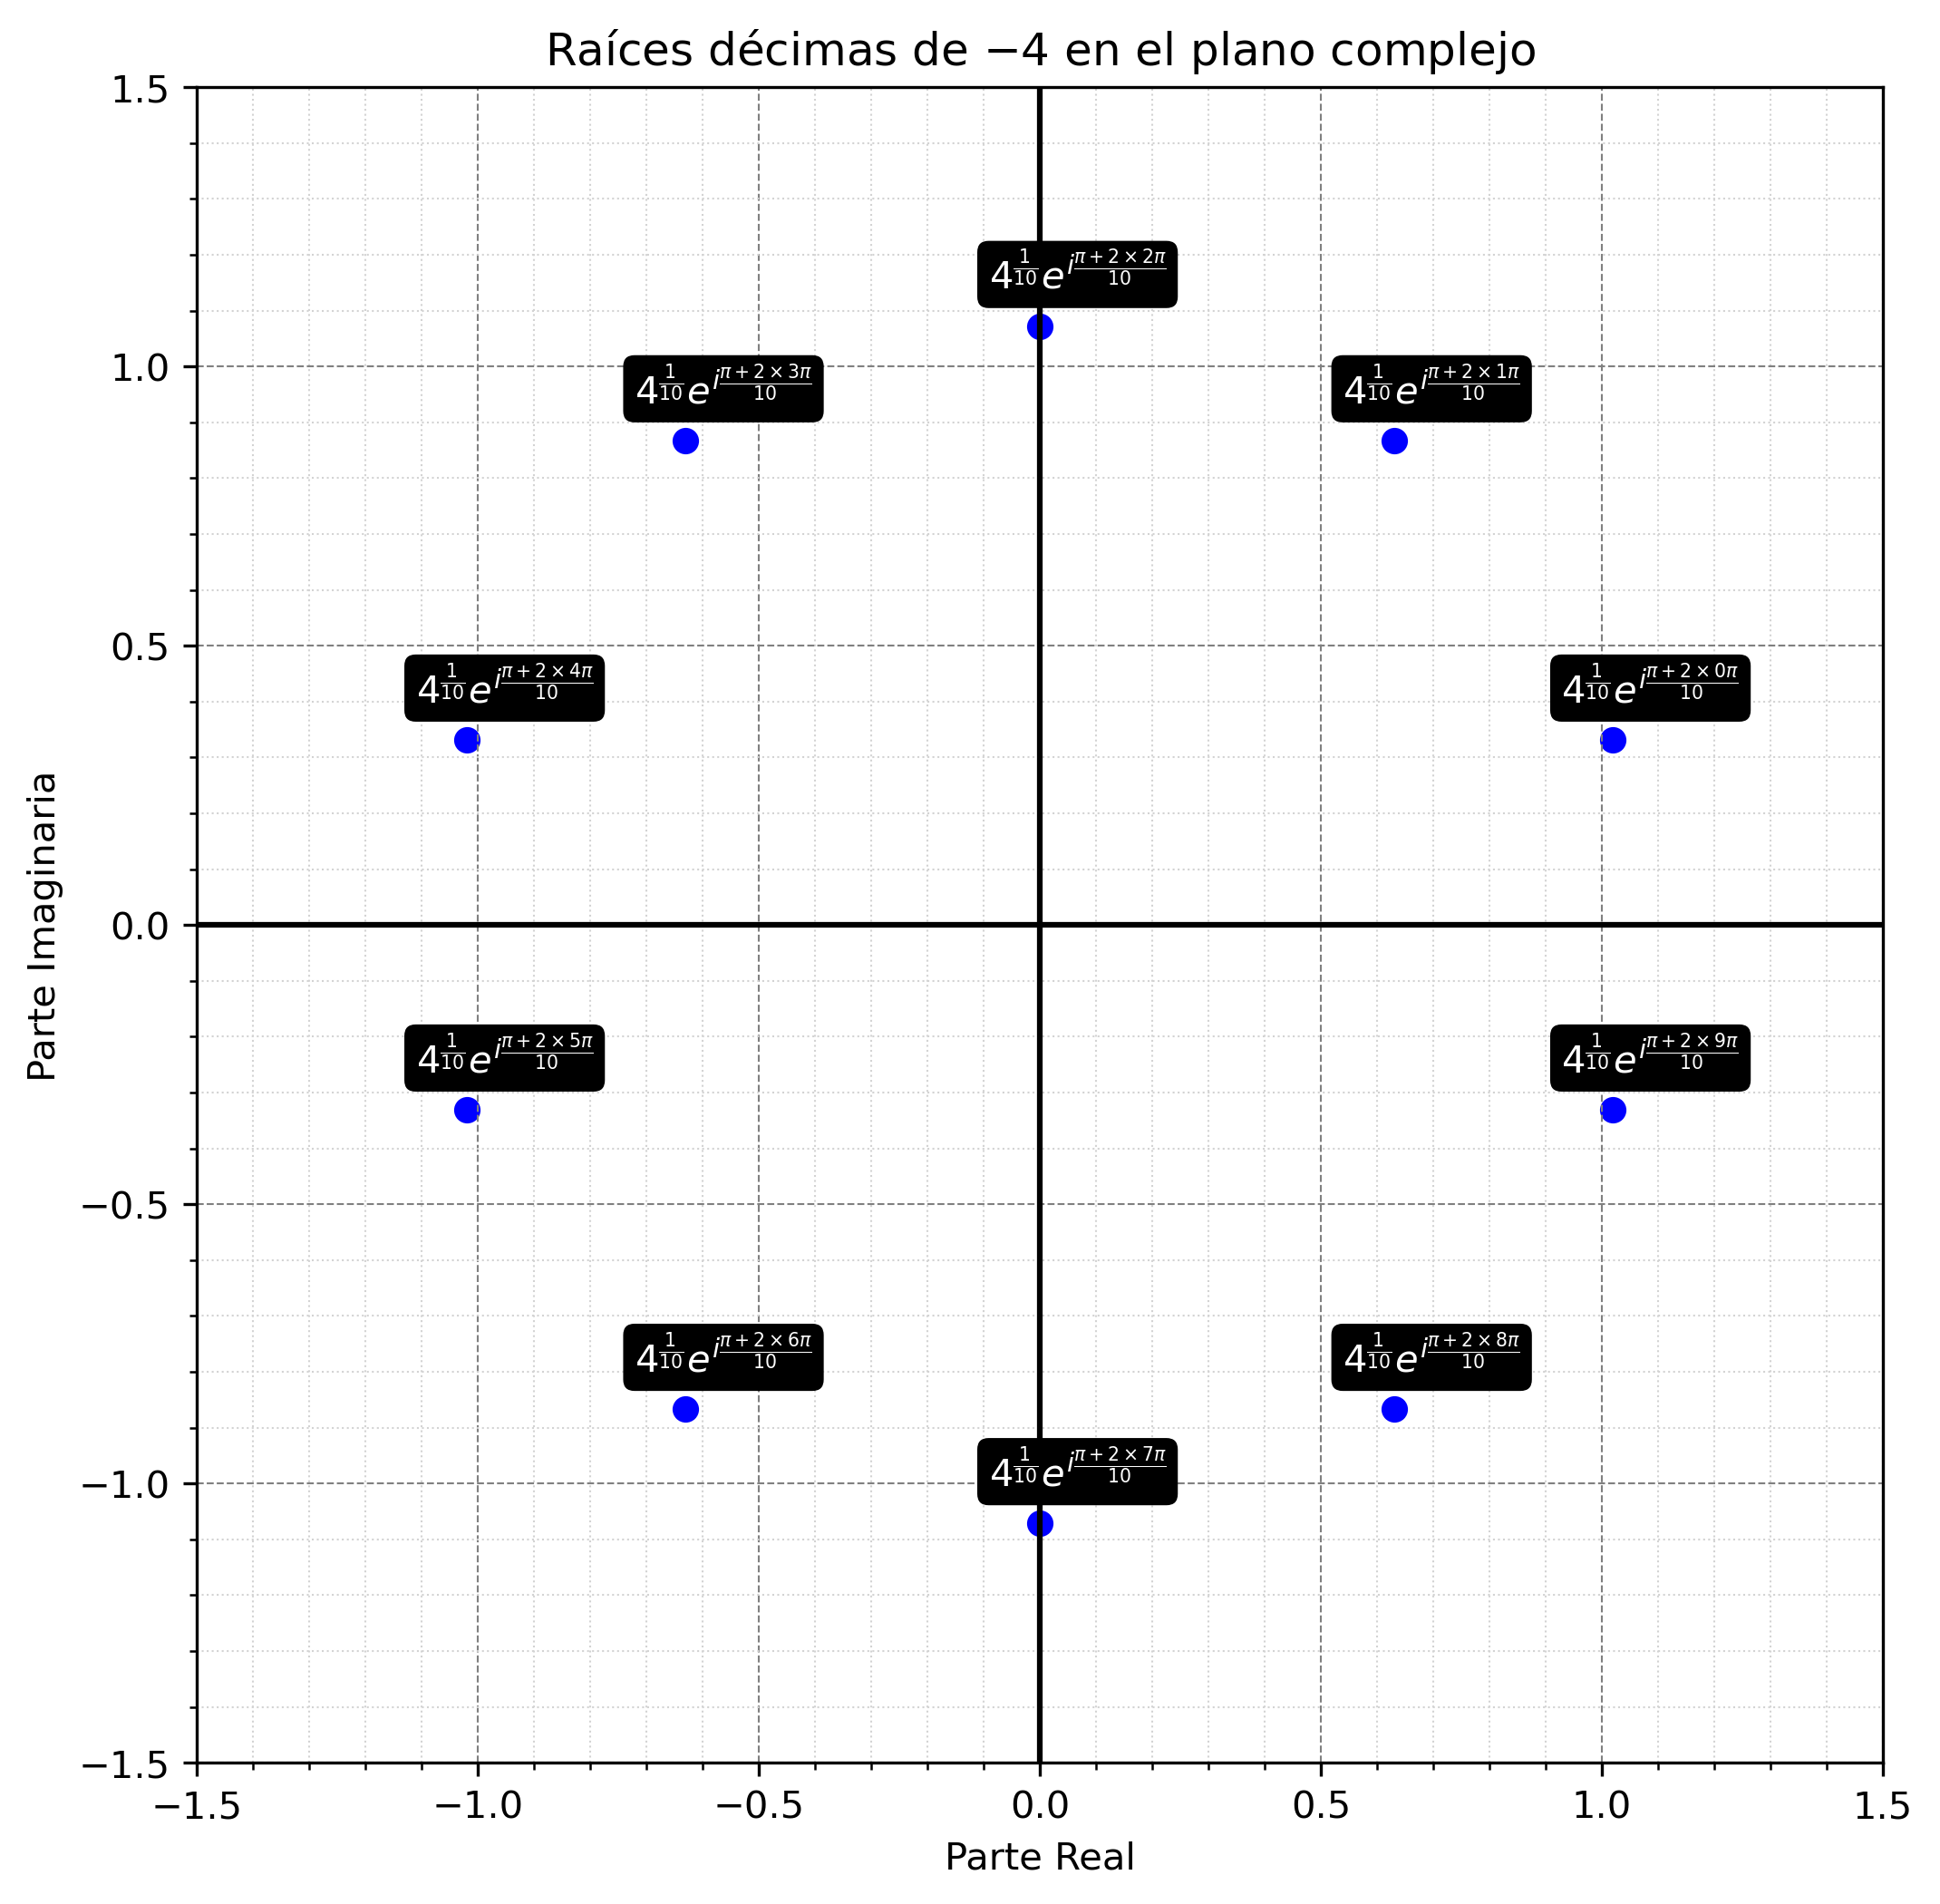
\includegraphics[scale=0.4]{images/grafico_raices_decimas_-4.png}  
    \end{center}
  \end{solution}
\end{homeworkProblem}
